% Alta forventer vekst på omtrent 50% personer over 67 i 2010-2020 og
% tilsvarende for de over 80 i 2020-2030.
% http://www.mynewsdesk.com/no/telenor/pressreleases/knytter-trygghetsalarm-til-pasientjournal-907498
% Fakta: Eldrebølgen, nordmenn over 67 øker fra 650k i dag til 1 mill før 2030
% Norge bruker 250 mrd på helse og sosialsektoren, eller 12% av BNP
% Utgiftene til sykehjemsplass er 850k i året, hjemmeboende er 200k
% SSB sykehjem øker fra 43k til 65k i 2030
% Sparing med velferdsteknologi: hvis 15-25% kan bo lengre hjemme sparer man
% 12-20mrd i 2030. Eller 40k årsverk som kan frigjøres.

% Sammendrag: Se
% http://nutsandbolts.mit.edu/Virtual_Ink/VirtualInk_Complete.pdf
% Sykt bra sammendrag... spesielt hvor mye penger vi trenger for å lage
% prototype.

% Se her!
% http://www.lister.no/phocadownload/helsenettverk_lister/2014_10_PA_rapport_om_alarmmottak.pdf
% Skrevet på oppgrad av helsedirektoratet... ser ut som SOS International er
% største leverandør. Det er et dansk firma tror jeg.

% GPS-skriv/studie fra SINTEF, de bruker safecall, for demens
% Kan ringe opp og lytte uten at noen vet det!
% http://www.sintef.no/globalassets/upload/konsern/trygge-spor-rapport_enkle-sider_lav-opplosning-2.pdf

% GPS: Lov å bruke GPS etter 2013 for denne typen tjenester, se
% https://www.stortinget.no/no/Saker-og-publikasjoner/Vedtak/Beslutninger/Lovvedtak/2012-2013/vedtak-201213-062/

% VIKTIG: Ta med i SKISSEN, at vi trenger å finne et passsende første produkt
% som bruker vår teknolog, slik det henger sammen med det som kommer etterpå.

% Første setning i sammendrag bør være ekstremt fengende: "Dagens
% mobilløsninger er avleggs, for de utnytter ikke no-install/nyeste versjon NÅ
% som man er vant med på internett <- gjelder altså fysiske devicer"

% Om produkt: Viktig å si "konkurrente kan IKKE endre funksjonalitet uten å
% danne en gruppe som skal sette seg ned og utvikle en prototype, fikse alle
% feil til de får det bra nok, søke godkjenninger, produsere selve driten og
% SÅ, etter ett år, kan de begynne å selge på markdet. Vi kan begynne å lage ny
% funksjonalitet på fredag og gjøre det tilgjengelig over nettet for ALLE
% brukerne våre på mandag."

% LES DENNE:
% http://www.uio.no/studier/emner/matnat/sfe/ENT4000/v12/undervisningsmateriale/04%20Forretningsplan%20Hansen.pdf
% Har glemt helt ut nettverk, det er viktig! Hva med konferanser, foredrag?
% Kapital, trnger vi ofte seff. Kjempegode tips her, spesielt grafisk eksempel.
% Redusere teknisk språk, spesielt i introen. Viktig med skalerbarhet! (det har
% vi, men må gjøres tydelig, spesielt VIS at vi har transformert problemet til
% å utvikle ny software, vi utviklet hardware bare én gang).
% Lyst å nevne planned obsolesence noe sted, hvor det passer.

% DIVERSE NOTATER
%
% Nitec, fins i stavanger, nitec.no. Kjempebra partner for utvikling.
% De selger faktisk trygghetsalarm med gsm i, men ser ut til å være stasjonær.
% Sier at analoge linjer skal legges ned, derfor trengs nye løsninger! <--- MÅ
% TAS MED! Opps deres løsning kan faktisk progges over nett, men har ikke
% display. Ser ut som de kjøper av caretech, gjør dem mer aktuell som partner.
% Skal vi selge til dem eller direkte? Vi ønsker å selge så direkte som mulig.
% Skal ha vertikalisering. Caretech er et svensk firma tydeligvis.
% De har gsm sak, men ser ut som en stasjon likevel, og små sensorer på
% armbånd, men de har falldetektor. Da må vi bare ha en liten støtsensor, men det
% koster jo litt med utviklingen. Ser også de tilbyr en rekke sensorer som man
% kobler opp mot sentralen, derav denne typen løsning. Dette kan vi tilby på
% sikt, men da at hver sensor er selvstendig, for eksempel. eller samma det.
% Hver bruker har forskjellige behov. Vet at mormor til Siri kun hadde
% alarm på hånden. De har knapp, lyser når den tar kontakt og blinker når den
% har kontakt. Så det er faktisk ikke rett fram det heller.De nevner overfall,
% innbrudd, personalknapp. Har batteriovervåkning, dette må vi også ha. Har
% tydeligvis batteri og kan ikke lades. Det er eneste ulempe med oss, må lade
% den hver natt. Kan være noen glemmer å ta den på. Løses ved at den sjekker om
% det er morgen, feks se når brukeren vanligvis står opp, og gir beskjed med
% hyling om den ikke er tatt på. :) De kjører IP67, så vi har jo en utfordring
% der, men det er bare vannavstøtende og ikke vanntett.
%
% Herlighet, se på lfh.no. Det er jo et sykt bra poeng at eldregruppen bare
% øker og øker, og vi forventer en eksplosjon på det området nå. Alle prognoser
% viser at det forventes sykt mye mer nødvendighet for hjelp. lfh.no sier i
% http://lfh.no/wp-content/uploads/2013/09/LFH-Tallfakta-kommune-WEB.pdf at man
% forventer at 380k personer vil ha behov for hjemmetjenester i 2040.
% Nivå for driftskostnader var 85 milliarder kr i 2012... Forventet i bli 147
% mrd i 2040. "Konsekvensene av eldrebølgen forventes å eskalere i 2020..."
% sier den saken. Derfor anbefaler LFH at Staten investerer i innovative
% løsninger allerede i dag.
% Hjemmetjenester er en del av primærhelsetjenesten i Norge (sykehus, osv).
% Vi opererer i markedet for hjemmetjenester.
%
% Konkurrenter: Moreto, gjort akkurat det vi vil, men på en annen måte
% http://www.tu.no/it/2013/01/27/nordmenn-gjor-trygghetsalarmen-tryggere
% Vi må omposisjonere oss litt pga dette. Foreslår biligere device, men dyrere
% månedsabb (de har andre priser for bedrift). Spørs om vi ønsker å konkurrere
% på pris, for det vi vil er å få enheten ut, for den kan kanskje brukes til
% BPA også.
%
% Se også skjema fra SINTEF, som bør bli partner:
% https://www.safemate.no/wp-content/uploads/2015/04/Skjema-for-vurdering-av-lokaliseringsteknologi-Safemate.pdf
%
% Må også satse på IP67 og A-GPS om en går på features.
%
% Se http://www.energibransjen.no/default.asp?menu=2&id=3908
% Moreto EDB gikk konkt, så kjøpte Lyse Smart konkursboet.
% Utfasing skjer 2017 og innen da må alle kommuner ha kjøpt nye alarmer som er
% på digitalt nett. Vår bør kunne kjøre på wifi også, forøvrig, og ha
% bluetooth, bare for å være bedre.
%
% Se her:
% http://www.ivarjohansen.no/temaer/sosialpolitikk/5198-trygghetsalarm-ogsa-for-fattigfolk-nei-bare-dersom-du-er-kredittverdig.html
% Kunne vært kult å subsidiere til slike personer, via firmaet selv?

% 110-telemark, se
% http://www.konkurransetilsynet.no/iKnowBase/Content/422277/A2006-44%20-%20Hjelp%2024%20Trygghetsalarm%20AS.pdf
% Klage fra hjelp24. Ble avslått.

% Mambo2 fra securinett tilbyr noe mer a la det vi vil lage
% http://www.securityworldhotel.com/no/Nyheter/Produktnyheter/securinet-presenterer-ny-trygghetsalarm#.VU0Bpc5K7i4
% Ser drit ut, men er der jaffal. Er DYR.

% Aleris vant kontrakt med telenor,
% http://www.nhoservice.no/article.php?articleID=5475&categoryID=329
% Viktigste er at det står at monopolet skal oppheves der i Oslo.

% Er mye konkurranse her, ass!

\chapter{Forretningsplan}

\textit{Mens vi i prosjektskissen tok utgangspunkt i \textit{<<The Business
Model Canvas>>} \cite{osterwalder} vil vi her sammenfatte elementer fra
Innovasjon Norge sin mal for forretningsplan \cite{innovasjon.norge}.}

\textit{Merk at vi også har forandret fokus. Etter vi leverte prosjektskissen
  fant vi ut at den opprinnelige idéen ikke var økonomisk holdbar. Vi har
  derfor valgt å satse på trygghetsalarm som et konkret produkt, bygget på
  toppen av konseptet i prosjektskissen. Detaljer finnes i kapittel
\vref{prosessen}.}

\section{Forretningsidé}

Mennesker i Norge lever stadig lengre, og vi forventer en økning i personer
over 67 på 17\% i 2030 og 21\% i 2050 fra vel 700 tusen i dag
\cite{org.alarmmottak}. Man forventer dermed en betydelig økning i kostnader
relatert til helsetjenester \cite{lfh.innspill}.

For å håndtere eldrebølgen på en human og økonomisk effektiv måte må vi finne
nye løsninger. \textit{Velferdsteknologi} er hjelpemidler som blant annet gjør
at eldre kan klare seg bedre selv, og bo lenger hjemme.

Én slik teknologi er \textit{trygghetsalarmen}. Ved å bære en sender med
alarmknapp rundt håndleddet eller halsen kan man tilkalle hjelp fra
hjemmesykepleiere ved akutte medisinske tilfeller.

Imidlertid har dagens løsninger svært begrenset funksjonalitet: Halvparten
krever en hussentral, og kan dermed ikke brukes ute (tabell
\vref{table.konkurranse.funksjoner}) eller til lokalisering av brukergrupper
som demente. I Sverige er det også få kommuner som tilbyr lokalisering
\cite{sverige.alarm}.

Hjemmesykepleiere sliter med effektiv organisering. Eksisterende produkt ringer
opp en vaktperson som da må ringe kollegaer for å finne én som er ledig for å
besøke brukeren.  Siling av alarmer, som har vist seg å være til stor hjelp i
utlandet \cite{org.alarmmottak}, er heller ikke mulig: Kun én av dagens
trygghetsalarmer har skjerm, og den brukes ikke som interaksjonsflate.

Vår forretningsidé er å bygge en moderne trygghetsalarm som dekker alle disse
behovene. Det skal være en mobil alarm som bæres rundt håndledd eller hals,
både inne og ute, og ha tilsvarende muligheter som smarttelefoner
\cite{alarmparadokset}.  Ved å utnytte tynnklientløsningen, som beskrevet i
prosjektskissen, kan vi redusere antall komponenter slik at vi kan selge den til
en pris tilsvarende konkurrentenes.  Ved å flytte kompleksiteten over til
tjenere \cite{mobil.virt.fordel} kan vi tilby \textit{ny} funksjonalitet til
eksisterende brukere med en momentan programvareoppdatering.

Da vårt produkt har en skjerm kan vi også tilby siling. Mens noen brukere kun
trenger én alarmknapp, kan andre få tilgang til å velge hva slags type alarm
som skal utløses. Da kan vaktsentralen se om det er snakk stell, eller et akutt
behov for øyeblikkelig hjelp.

Enheten skal også selges til hjemmesykepleiere. En alarm kan da rutes til de
nærmeste hjemmesykepleierne. Ved aksept av anrop kan både bruker og kollegaer
få vite hvor langt vekke hjelpen er.

\textbf{Vår visjon er å bli en ledende, global leverandør av avanserte
velferdsteknologiske løsninger som effektiviserer helsetjenesten og gir eldre
større trygghet og selvstendighet til å bo hjemme lengre.}

\section{Forretningsmodell}

Forretningsmodellen vår er å selge utstyr direkte til hjelpemiddelsentraler,
til samme pris som konkurrentene, men ta mer betalt månedlig for datatrafikk og
skytjenester.  På sikt skal vi tilby ny funksjonalitet gjennom oppdateringer
over nettet, på samme maskinvare, for alle brukere.

\subsection{Kundesegment}

Kundemassen vår er todelt: Hjelpemiddelsentraler på fylke- og kommunenivå, og
leverandører som kan videreselge vårt produkt.  Vi har også en brukermasse
bestående av primært eldre mennesker med behov for alarmer, trygghet og
brukervennlighet, og hjemmesykepleiere som skal kunne svare på
alarmoppringninger.  Vi ser bort fra privatmarkedet, da dette vil stjele tid og
energi vi kan bruke på innsalg til det offentlige.

Eksisterende trygghetsalarmer mangler i stor grad tilkobling til internett, få
er mobile ogde er ikke mobile, med mindre man har ekstrautstyr, og mangler
oftest GPS \cite{sverige.alarm}.  Det oppleves også mye feil med alarmene,
og de må kontrolleres manuelt. Dette skjer i snitt én gang per døgn. Når Norge
er blant de fremste i verden på å ta i bruk velferdsteknologi
\cite{telenor.undersokelse} regner vi med tilsvarende behov i utlandet, men vi
skal bygge opp renommé og tillit i Norge i første omgang.

Hjelpemiddelsentralen vil vektlegge produkter som fungerer og seriøse,
forpliktede leverandører. Mer avanserte tjenester som GPS forutsetter god
organisering \cite{org.alarmmottak}.

\subsection{Verdiløfte}

Vårt verdiløfte er å levere en trygghetsalarm med moderne funksjonalitet på
nivå med smarttelefoner som kan øke brukerens opplevelse av trygghet gjennom
raskere responstid og dermed effektivisere tidsbruken til hjemmesykepleiere.

Betalingsvilligheten anses som å være høy, da de eksisterende tjenestene er
relativt dyre, selv om funksjonaliteten som tilbys er laber.  SOS International
legger for eksempel på 245 kr i måneden for brukere som ønsker en ekstra
alarmknapp\footnote{Riktignok for privatkunder.} \cite{sos.int}.

\subsection{Distribusjonskanaler}

% • Hvor eller på hvilken måte leverer/distribuerer bedriften sine
% produkter/tjenester ? 
% • Hvilke kanaler brukes for å kommunisere/markedsføre kundeverdi og fortrinn ?

%%%%%%%
% MERK: Dette går mer på levering, distribusjon, ikke salg. 
% Kjøper hver kommune inn dette? -> er per fylke. De har sikkert kjempelyst til
% å spare penger.
%%%%%%%

Salg skjer direkte til hjelpemiddelsentraler på tradisjonelt vis, ved å sette
opp møter, demonstrasjoner og sender større forsendelser per post. Vi skal også
selge gjennom leverandører for å øke brukermassen.

Kommunikasjon skjer gjennom telefon, hvor vil vil sette opp støttepersonell med
tilhørende vakttjeneste utenfor kontortiden.

Markedsføring skal skje gjennom deltakelse og presentasjoner på konferanser,
gjennom bransjeblad og <<on-site>> demonstrasjoner.  Vi skal også ha en tydelig
tilstedeværelse på nett, optimalisert for bestemte søkeord.

\subsection{Kunderelasjon}

% • Hvordan bygges kunderelasjoner?
% • Hvordan opprettholdes gode kunderelasjoner over tid?
% • Hvem er dine viktigste konkurrenter?
% • Når og hvorfor blir disse valgt?

% Hvem er egentlig kundene? Privatkundet har vi nevnt, og partnere, men virker
% som det egentlig er hjelpemiddelsentralen. Skal vi selge dette selv til
% hjelpemiddelsentralen? De vil nok ha flere tjenester enn den vi har, ting som
% kan kobles sammen.
% - Definitivt selge direkte til privatkunder
% - Definitivt selge ti hjelpemiddelsentralen, men de vil nok ha andre typer
%   sensorer også. Det gir mulighet for å lage flere produkter, gitt vi har
%   suksess for de andre. De har folk som kun har trygghetsalarmen og ikke noe
%   mer enn det. Blir fort utvikling av røykvarslere også.
% OK, ser ut som det blir to kunder: Privatpersoner og kommuner. Kommuner deler
% ut alarmene. Hvem betaler for dem? Kjøper disses inn per kommune?
% Er ihvertfall kommunene som tar regningen, enten delvis eller helt (feks
% Meldal).

Den viktigste faktoren for å bygge kunderelasjon er ved å skape tillitt. Tillit
til at vi er profesjonelle og at produktet virker som det skal. Vi starter i
det små med demonstrasjoner og vil prøve å få til et pilotprogram. Det skal
være grobunn for tillit og senere salg.

At vi blir ansett som seriøse og forpliktet til vår visjon er kritisk.
Konkurrentene er store aktører med mange ansatte og lang fartstid i markedet.
Det er derfor lett å velge dem som leverandør, fordi risikoen er lav.
Vi må dermed begynne i det små og bygge opp et godt ry, bit for bit.

\subsection{Inntektsstrøm}

% • Hvordan skapes inntekter fra kjernevirksomheten?
% • Hvordan oppnås eventuelt andre inntekter?

Inntekter genereres ved utstyrssalg og månedlig betaling for bruk av
tynnklientsystemet. Andre inntekter skapes ved å utvikle nye funksjoner og
selge dem som oppdateringer. Eksempler er medisinalarm, elektronisk gjerde,
språk- og kulturtilpasning, avviksrapportering med mer. Strategien utover dette
er å komplettere tilbud med sensorer for røykvarsling, innbrud og lignende. Vi
vil også vurdere muligheten for å gå inn i andre nisjemarkeder som for eksempel
styringspaneler for automater, alarmsystemer og taksameter.

\subsection{Nøkkelressurser og kritiske suksessfaktorer}

% • Hvilken gjennomføringsevne har bedriften?
% • Kompetanse og personlige egenskaper som gjør deg/dere spesielt egnet til å
% utvikle og drive bedriften?
% • Hvilke viktige ressurser og tilleggs-kompetanse trenger bedriften …
%    o på kort sikt?
%    o på lenger sikt?
% for å realisere forretningside og kundeverdien (“verdiløftet”)?

% TA MED: At vi blir sett på som seriøse, at vi har kraft og kapital og antall
% ansatte til å dra driften, kommunene satser nok vanskelig på de man anser som
% korttidslevede (flyktige). Tillitsbygging er viktig, men det kan vi bare
% gjøre over tid (fra bioenergi).


Vi har lang erfaring med å bygge programvare for driftskritiske systemer, også
innenfor helsesektoren, hvor vi har laget timepåminnelser for sykehus som AHUS.

Vi trenger domeneeksperter på velferdsteknologi, personer som har erfaring med
offentlig innsalg og kvalitetssikring av elektroniske produkter.

% Kort sikt: Hardware-eksperter, offentlig salg, direktiver og regler,
% domeneeksperter
% Lang sikt: Global handelsrådgivere, økonomer for hvordan optimalisere
% inntjening når vi er igang, markedsføring for å vise oss igjen. I første
% omgang skal vi bare bevise at vi har livets rett, men snart må vi bevise at
% vi har rett til overleving. Trenger mobileksperter.

% Hva slags tilleggskompetanse trenger vi: 

% Hva er forskjellen på partnere og nøkkelressureser?
% Kritiske suksessfaktorer: Fungerende prototype, pilotprogram, første salg,
% første inntekt.
% Designere, må ha noen som kan lage dette

\subsection{Kjerneaktiviteter}

% • Hvilke kjerneaktiviteter må bedriften selv utføre?
% • Hvilke (kjerne-) aktiviteter kan/må settes ut til andre?
% • Hva er de mest kritiske faktorer for å lykkes mht lønnsom kommersialisering?

Vi må selv utvikle prototype for alarmen og tilhørende tjenerplattform.

Produktdesign gjøres gjennom oppdrag av profesjonelle. Komponentene er
hyllevare og monteres på kretskort av eksterne bedrifter. Ved skalering bør de
også sette sammen det endelige produktet. Testing gjøres av oss. Tjenerparken
leies som skytjenester og skaleres etter behov. Revisjon og det juridiske
utføres av konsulenter.

Kritisk for suksess er at prototypen virker, er pålitelig og lett å bruke, at vi
får til et pilotprogram med en eller flere kommuner og at vi imøtekommer
nødvendige godkjenninger og direktiver for elektroniske produkter.

\subsection{Partnere}

% • Hvilke partnere og leverandører samarbeider bedriften med for å kunne levere
% på sitt verdiløfte (2)?
% • Hvilke er avgjørende viktig på kort og på lenger sikt?

\textbf{Innovasjon Norge} er en naturlig partner for rådgivning i
oppstartsfasen. De kan også hjelpe oss på lengre sikt dersom vi satser globalt.
Da trengs det kunnskap om internasjonal forretningsjus, så vel som lokal, kulturell
kjennskap.

\textbf{Universiteter} med utdanning innenfor helse og teknisk design kan
hjelpe oss med utvikling og forskning, spesielt gjennom studentoppgaver.


Halvparten av de norske aktørene produserer ikke utstyret selv. Ved å danne
partnerskap til noen av disse kan vi utnytte deres markedskunnskap og nettverk.
En potensiell partner er \textbf{Nitec}, som er basert i vårt nærområde.

\textbf{SINTEF} kan brukes til godkjenninger, kvalitetssikring, utprøvelse og
generell forskning. Dette gjøres ved å søke om et \textit{innovasjonsprosjekt i
næringslivet} (IPN) til Forskningsrådet.

\section{Marked}

% Beskriv ditt marked
% Vær så konkret som mulig
% Hvor stort er det og hvordan vurderer du utviklingen i markedene?
% Dersom du har gjennomført en kunde- / markedsundersøkelse, legg ved en
% beskrivelse og resultatene

% Konkurrenter:
% Hvem er de viktigste konkurrentene?
% Hvilke styrker og svakheter har de?
% Hvordan oppfattes de i markedet?

% TODO: Oppdater markedspris
Med et marked på 300 millioner kroner i Norge (beregning i kapittel
\vref{marked}) er det likevel mange konkurrenter.

Kommunene er interesserte i store, seriøse og pålitelige aktører som gjerne
tilbyr flere tjenester.  For eksempel vant Aleris nylig en kontrakt på levering
av 3200 alarmer i Oslo \cite{telenor.aleris}, men de tilbyr ikke avanserte
tjenester. Effektivisering og kostnadsbesparelse er også viktig. I Skien kan
alle med brannvarslingsoppkobling få trygghetsalarm fra 110-Telemark
\cite{telemark.konkurransetilsyn}, som forøvrig også ble rapportert til
Konkurransetilsynet.

\subsection{Vekstmål}

Målet vårt er å ta 10\% av markedet i Norge på fem år.

% Beskriv hvorfor du/dere ønsker å etablere/utvikle egen bedrift
% Hvilke (vekst) ambisjoner foreligger – på kort og lenger sikt (tallfest)

For å skape tillit til bedriften og produktet, ønsker vi å starte med en liten
masse på 500 brukere.

Dette skal bli grobunn for å selge via leverandører som kjøper utstyret fra
andre produsenter (tabell \vref{table.konkurranse.funksjoner}).  Vi skal vinne
dem over med bedre teknologi, flere funksjoner og svært gode innkjøpspriser: Vi
har høy dekningsgrad på alarmene og tjener inn avslag på månedlig abonnement
(tabell \vref{table.drift}).  Dette skal øke brukermasen til 1500 og 2500 på
tre år (tabell \vref{table.driftsbudsjett}).

Målsetningen for det fjerde året er 4000 brukere. Det skal vi nå med en
kombinasjon av jevn markedsføring, opprettelse av nye utprøvingsprogram og
organisk vekst \cite{bessant}.  Budsjett for markedsføring økes ytterligere det
fjerde året for å komme opp på 7000 brukere ved utgangen av det femte året.

\subsection{Konkurrenter}

% Finnes liknende produkt/tjeneste på markedet?
% Finnes liknende løsning eller prosess på markedet?
% Har bedriften søkt patent eller annen form for beskyttelse? Evt hvorfor ikke?
% Er det andre patenter som kan innvirke på bedriftens forretningspotensiale?

Dignio selger den svensk-produserte Doro seniortelefonen som trygghetsalarm.
Dette er det eneste produktet på markedet som er i nærheten av vårt konsept.
Den har GPS og kan oppdateres med ny funksjonalitet over nettet, men skjermen
er ikke den primære interaksjonsflaten: Det er en klapptelefon som skal brukes
lukket, men en alarmknapp på baksiden.

Vi har ikke søkt patenter men bør bygge opp en portefølge for beskyttelse i
helsemarkedet \cite{slides.chery}.  Det finnes svært mange patenter på
virtualisering, mobilteknologi, tynne klienter og alarmer
\cite{patent.ricordi2008mobile, patent.heinz2013wearable}. Disse må kartlegges
i forkant av utviklinsoppstart. Vi har budsjettert med generell rådgivning men
ikke medregnet lisenskostnader.

\begin{table}
  \centering
  \begin{tabular}{lccccc}
    \textbf{Navn} &
    \textbf{Produsent} &
    \textbf{Utendørs} &
    \textbf{GPS} &
    \textbf{Skjerm} &
    \textbf{Apps} \\

    %Navn              %Pr %UTE %GPS %Skj %Apps
    Safemate (bedrift) & J & J  & J  & N  & N \\
    Careto (TR-203)    & J & J  & J  & N  & N \\
    Careto (Pico)      & J & J  & J  & N  & N \\
    NUMA (TA10)        & J & N  & N  & N  & N \\
    Nitec (CareIP)     & N & N  & N  & N  & N \\
    SOS International
    (Trex)             & N & N  & N  & J  & N \\
    Sos International
    (Neo)              & N & N  & N  & N  & N \\
    Dignio
    (CareTech Doro)    & N & J  & J  & J  & J \\
    \textbf{Vårt produkt}
                       & J & J  & J  & J  & J \\
  \end{tabular}
  \caption{Konkurrenters funksjoner}
  \label{table.konkurranse.funksjoner}
\end{table}

\subsection{SWOT-analyse}

Vår styrke er moderne teknologi med berøringsskjerm, ettersalg og en
effektiviseringsløsning. Utnyttelse av dette er allerede beskrevet.

Svakhetene våre er en kompleks totalløsning, ukjent batterikapasitet og høyre
krav til oppetid og sikkerhet. Dette kan kun løses gjennom testing og erfaring
fra pilotprogram.

Muligheter på markedet er å heve kommunenes forventninger til denne
produktkategorien gjennom bedre teknologi, spesielt på effektivisering. Men vi
er truet av at markedet kan være mettet, det er tidkrevende å komme på markedet
med utvikling, testing og direktivgodkjenning. Hvordan utnytte
lokaliseringstjenester er heller ikke klart \cite{sintef.trygge.spor}.

% Merk også, mange bruker alarmen bare når de skal ha hjelp til noe trivielt,
% feks å vaske opp søl på gulvet, og sånt. Vår sak MED SKJERM (har bare sett 1
% konkurrent som har det, MAMBO2) kan faktisk man skrive sånt, slk at
% sykepleiere kan prioritere. Kanskje også lurt om vi utvider på web-siden slik
% de kan gjøre mer ting, feks integrerer med eksisterende systemer,
% vaktsystemer osv. Ved hjelp, kult om en kan bare rope høyt og så varsler den.
% Perfekt hvis man ikke klarer å nå knappen men faller eller får
% epilepsianfall. Hadde også vært kult med hearbeat sensor eller noe sånt.

% Cite regler for offentlig anskaffelse:
% https://www.regjeringen.no/nb/dokumenter/veileder-offentlige-anskaffelser/id437022/
% Cite gjerne de som gikk konk (Merito) ifbm seriøsitet/overlevelsesdyktighet.
% TIpper kommunene ser mye på det. Tror også det er lett å bli bedre på
% funksjonalitet, men det er mange, så tror ikke det er det de primært ser
% etter. Det de trenger er jo bare den knappen.

% Generelt vil jeg frem til: Det vi må satse på er masseavtale, altså lage en
% avtale som leverer for et helt fylke eller kommune. Må utnytte partnere
% (domeneeksperter, SINTEF, feks). Høy konkurranse kan vi snu til en fordel med
% at vi henvender oss til de som sitter med kunnskap men ligger bak. De bør
% være kjempeinteressert i teknologi. Pris, med vår teknologi kan vi lage noe
% som gjør at vi har mye å gå på når det gjelder pris. Å havne i priskrig er
% ikke så lurt, men vi har mye å gå på. Derfor begynner vi med å si at
% enkeltpris er omtrent lik de andre, men hvis vi kjøper i volum så slår vi
% VELDIG mye av på årisen, bruker altså opp marginhøyden på dette.
% Offentlige anskafelser er vanskelig, men merk 110-Telemark, vi kan faktisk
% kanskje få til noe lignende. Vi kan jo vise til telemark, dette blir uansett
% bare en lokal strategi, funker ikke på nasjonalt plan og er et juridisk
% minefelt hvis vi gjør feil. Patenter kan også beskytte oss til en viss grad.
% Vi bør i hvertfall ha noen sentrale som kan brukes, selv om vi bare vil bruke
% de som beskyttelse, ikke offensivt (for det koster penger).
% At markedet er mettet, er vår løsning så mye bedre enn det vi har? Tror det
% går mye på faktisk oppsett og hva de opplever av oppetid.

% Grupper først per del og så skriv om gruppen.
% Hvordan styrke sterke sider:
% Hvordan redusere svakheter: Rundt halsen, testing, pilotprogram

% Hvordan utnytte muligheter: Grupper: Pris, teknologi, funksjonalitet
% Må vise at det funker med et pilotprogram og anbefalinger.
% Må vise at man kan spare penger på dette.

% Hvordan avverge trusler: Grupper: marked, regler, status quo
% Utnytt konkurranse ved å henvende til de som ligger
% på 2. plass. Offentlig anskaffelse er et problem, m

% TODO: Skriv tekst om hvordan gjøre det under.
% Hvordan:
% - Styrke sterke sider
% - Redusere svakheter
% - Utnytte muligheter
% - Avverge trusler

\section{Økonomiske forhold}

\subsection{Produktkalkyle}

Kostnaden for å produsere én alarmenhet er gitt i tabell
\vref{table.pris.alarm}.  Delepriser er tatt fra nettstedene til \textit{Mouser
Electronics} og \textit{Qualcomm} og volumpriser er \textit{beregnet} basert på
andre komponenter vi fant der.

\begin{table}
  \centering
  \begin{tabular}{lr}
    \textbf{Del} & \textbf{Volumpris} \\
    CPU / GPU / GSM SoC & 58,40 kr \\
    RAM       & 10,95 kr \\
    ROM       &  3,65 kr \\
    Batteri   &  7,30 kr \\
    Skjerm    & 29,20 kr \\
    Lyd I/O   &  5,84 kr \\
    Annen elektronikk & 58,40 kr \\
    Ikke-elektroniske deler & 58,40 kr \\
    Montering og testing & 7,30 kr \\
    \textbf{Sum} & \textbf{239,44 kr} \\
  \end{tabular}
  \caption{Enhetsproduksjonskostnad for alarm.}
  \label{table.pris.alarm}
\end{table}

\subsection{Kostnadsstruktur og driftsbudsjett}

% • Hvilke kostnader vil bedriften ha for å utvikle og drifte sitt
% forretningskonsept?

Den største kostnaden for utvikling av produktet er lønn og deretter
datatrafikk (tabeller \ref{table.kostnad.alarm}, \ref{table.driftsbudsjett} or
\ref{table.drift}).  Mesteparten av utviklingen kan gjøres på vanlige
datamaskiner, og komponentene er billig hyllevare. Det er også satt av kapital
for å sørge for at produktet følger gjeldende EU-direktiver for elektroniske
produkter \cite{dir.rohs, dir.2001.95}.


\begin{table}
  \begin{tabular}{lrrrrr}
   & \textbf{1.~år} & \textbf{2.~år} & \textbf{3.~år} & \textbf{4.~år} & \textbf{5.~år} \\
    \textbf{Brukere} & 500 & 1500 & 2500 & 4000 & 7000 \\
    \\
    \textbf{Omsetning} \\
    Inntekt alarm   (eks. mva.)      &  800 & 1599 & 1599 &  2399 &  4798 \\
    Inntekt abonnement (eks. mva.)   &  955 & 2866 & 4776 &  7642 & 13373 \\
    \textbf{Sum}                     & 1755 & 4465 & 6375 & 10041 & 18171 \\
    \\
    \textbf{Variable kostnader} \\
    Produksjon alarm                &   120 &  240 &  240 &   360 &   720 \\
    Datatrafikk alarm               &   235 &  706 & 1176 &  1882 &  3293 \\
    Datasenter                      &    16 &   49 &   82 &   132 &   230 \\
    \textbf{Sum}                    &   371 &  995 & 1498 &  2374 &  4243 \\
    \\
    \textbf{Dekningsbidrag}         &  1384 & 3470 & 4877 &  7667 & 13928 \\
    \hline
    \\
    \textbf{Faste kostnader} \\
    Lønnsutgifter                   &  2544 & 2544 & 3392 &  3392 &  5936 \\
    Kontor                          &   144 &  144 &  144 &   144 &   576 \\
    Internett                       &    10 &   10 &   10 &    10 &    10 \\
    Regnskap og revisjon            &    75 &   75 &   75 &    75 &    75 \\
    Markedsføring                   &   100 &  100 &  100 &   200 &   100 \\
    Andre kostnader
    (strøm, reiser, m.m.)           &    30 &   30 &   30 &    30 &    30 \\
    \textbf{Sum}                    &  2903 & 2903 & 3751 &  3851 &  6727 \\
    \\
    \textbf{Dritfsresultat før avskrivninger}
                                    & -1519 &  567 & 1126 &  3816 &  7201 \\
    \hline
    \\
    \textbf{Avskrivninger} \\
    Datamaskiner (over 5 år)        &     7 &    7 &   10 &    10 &    17 \\
    \\
    \textbf{Årsoverskudd}           & -1526 &  560 & 1116 &  3806 &  7184 \\
    \thickhline
    \\
  \end{tabular}
  \caption{Driftsbudsjett over fem år (beløp i hele tusen kr).}
  \label{table.driftsbudsjett}
\end{table}


\begin{table}
  \centering
  \begin{tabular}{lr}
    Lønnsutgifter (2 personer, 1 år) &  1.696.000,00 kr \\
    Datamaskiner                     &     24.000,00 kr \\
    Komponenter og utstyr            &     10.000,00 kr \\
    Design deksel                    &     50.000,00 kr \\
    Teknisk rådgivning               &    100.000,00 kr \\
    Godkjenninger                    &    100.000,00 kr \\
    \textbf{Sum}                     &  1.980.000,00 kr \\
  \end{tabular}
  \caption{Kostnader for å utvikle trygghetsalarm.}
  \label{table.kostnad.alarm}
\end{table}

\begin{table}
  \centering
  \begin{tabular}{lr}
    \textbf{Forutsetninger} & \\
    \textit{Ansatte}                                           & \textit{4} \\
    \textit{Brukere}                                           & \textit{4000} \\
    \textit{Pris månedsabonnement (inkl. mva)}            & \textit{199,00 kr} \\
    \textit{Kostnad datatrafikk (100 Mb/mnd., inkl. mva.)}   & \textit{49,00 kr} \\
    \textit{Kostnad datasenter (1000 brukere/år)}            & \textit{32.913,27 kr} \\
    \textit{Kostnad kontorleie (1 $\text{m}^2$/mnd.)}        & \textit{400,00 kr} \\
    \\
    \textbf{Omsetning} & \\
    Inntekt abonnement (eks. mva.)                    &  7642 \\
    \\
    \textbf{Variable kostnader} & \\
    Datatrafikk alarm                                 &  1882 \\
    Datasenter                                        &   132 \\
    \textbf{Sum}                                      &  2014 \\
    \\
    \textbf{Dekningsbidrag}                           &  \textbf{5628} \\
    \hline
    \\
    \textbf{Faste kostnader}                       & \\
    Lønnskostnad                                      &  3392 \\
    Kontor             ($30~\text{m}^2$)              &   144 \\
    Internett                                         &    10 \\
    Regnskap og revisjon                              &    75 \\
    Markedsføring                                     &   100 \\
    Andre kostnader (strøm, reiser, m.m.)             &    30 \\
    \textbf{Sum}                                      &  3851 \\
    \\
    \textbf{Driftsresultat før avskrivninger}         &  \textbf{1777} \\
    \hline
    \\
    \textbf{Avskrivninger}                            & \\
    Datamaskiner (over 5 år)                          &    10 \\
    \\
    \textbf{Årsoverskudd}                             &  \textbf{1767} \\
    \thickhline
    \\
  \end{tabular}
  \caption{Driftsbudsjett (i tusen kr) for 4000 brukere, uten salg av alarmenheter.}
  \label{table.drift}
\end{table}


\subsection{Kapitalbehov}

Gitt utviklingskostnaden (tabell \vref{table.kostnad.alarm}) og
driftsbudsjettet (tabell \vref{table.driftsbudsjett}) har vi satt opp
kapitalbehovet i tabell \vref{table.kapitalbehov}.

\begin{table}
  \centering
  \begin{tabular}{lr}
    Utviklingskostnad   & 1.980.000,00 kr \\
    Underskudd 1.~år    & 1.526.000,00 kr \\
    Kapitalbehov 2.~år  &   966.000,00 kr \\
   \textbf{Sum} & \textbf{4.472.000,00 kr} \\
  \end{tabular}
  \caption{Kapitalbehov}
  \label{table.kapitalbehov}
\end{table}

Med et kapitalbehov på 4.472.000,00 kr så vil bedriften gå med totalt overskudd
innen fem år (tabell \vref{table.driftsbudsjett}).

\chapter{Analyse og diskusjon}

\section{Utvikling i arbeidsprosessen}
\label{prosessen}

I prosjektskissen beskrev vi en visjon om en helt ny type mobiltelefon, basert
på tynnklientkonseptet.  

Når vi imidlertid undersøkte dette i detalj fant vi ut
at gjennomsnittlig datamengde ville ligge på rundt 9--10 Gb per måned. Dette er
langt over det som er vanlig for både forbrukere og teleoperatører i dag, og
derfor er det uoverkommelig dyrt.

Deretter begynte vi å se på en ny produktkategori: Smartklokker. Hovedproblemet
her er å konkurrere med giganter som Apple og Samsung, og vi er forøvrig for
sent ute til å kunne være med å forme forbrukeres forventninger til denne type
produkt.

På dette tidspunktet begynte vi å konkretisere produktet mer. Tynnklienter
krever en døgnkontinuerlig tjenerpark, dermed må vi ta en månedsavgift for å
dekke driftsutgifter. Dessuten ville det være lurt å lage et relativt enkelt
produkt, sammenlignet med en smartklokke. Vi undersøkte bruksområder for hvilke
typer applikasjoner som behøver konstant tilgang på nett, nisjespesialisering og som passer inn i
abonnementsmodellen. Vi hadde flere alternativer, men trygghetsalarmen så ut
til å ha et skrikende behov for en ny vri. Dette gjorde arbeidet mye lettere.

Vi var også usikre på hvor mye strøm en tynnklient ville trekke på grunn av økt
trådløskommunikasjon, og dette er fremdeles et usikkerhetsmoment for
trygghetsalarmen.

Vi har altså hoppet frem og tilbake i innovasjonsprosessen presentert i
læreboka \cite{bessant}, akkurat slik som forventet.

Vi har forøvrig stor tro på vårt konsept, for en kan bruke samme maskinvare og
plattform til en rekke andre nisjeprodukter: <<Hands-free>> systemer for
industriarbeider, inkludert talestyrt plukking på Bama, styring og panel for
innbruddsalarmer i hus, taxi taksameter, grensesnitt på brusautomater og
lignende --- til og med grensesnitt for kassaapparat.  Hver produkttype krever
kun ny programvare på tjenersiden, og man kan oppnå <<economy of scale>> ved å
bruke samme maskinvare på en rekke områder.

Imidlertid er det en ulempe med dette, og det er at hver kategori krever
domeneekspertise. For å være seriøse må vi allokere mange folk per type produkt
og bygge opp kunnskap. Det er også nye separate markeder som vi er nødt å
tvinge oss inn i hver gang.


\section{Markedsanalyse}
\label{marked}

Grunnlaget for å estimere markedsstørrelse er tatt på bakgrunn av tall fra
Statistisk Sentralbyrå \cite{iplos.2013, ssb.trygghetsalarm}. Antall mottakere
av trygghetsalarmer er vist i figur \vref{fig.mottakere}. Her ser vi at antall
mottakere har holdt seg mellom 73--74 tusen de siste årene, men med historisk
økning.

% TODO: Ta med flyktige, mindre enn ett år, og vis til tabell og utregning.
Snittpriser på utstyr og månedsabonnement er henholdsvis 2.870,25 kr og 101,50
kr (tabell \vref{table.konkurranse.pris}). Dette er uten oppkobling mot
sentral.  Med 73 tusen mottakere gir det rundt 210 millioner kr for utstyret og
90 millioner per år i basisabonnement, altså et anslått marked på 300 millioner
kr.

\begin{table}[h]
  \centering
  \begin{tabular}{lrrr}
    \textbf{Navn} &
    \textbf{Utstyrspris (kr)} &
    \textbf{Abonnement per måned (kr)}\\
    Safemate (med lader) & 1.998,00 & 129,00 \\
    Careto (TR-203)      & 1.998,00 &  99,00 \\
    Careto (Pico)        & 2.995,00 &  99,00 \\
    NUMA (TA10)          & 3.990,00 &  79,00 \\
    \textbf{Snitt}       & 2.870,25 & 101,50 \\
  \end{tabular}
  \caption{Utstyrspris for trygghetsalarm}
  \label{table.konkurranse.pris}
\end{table}

Det faktiske markedet er nok noe høyere. For \textit{privatkunder} tar
\textit{SOS International} 951,00 kr i etablering og 7.154,00 kr per år. Dette
er med egen bemanningssentral og inkluderer utstyrskosten. Dersom de hadde
levert til hele landet som privatkunder ville det utgjort 522 millioner.  I
figur \vref{fig.mottakere} ser vi også at hvert år er det 20 tusen mottakere
som bruker alarm i en kortere periode. For \textit{privatkunder}, med sin egen
bemanningssentral, tar SOS International 3.770,00 kr for en periode opp til tre
måneder.  Dersom de hadde levert til 20 tusen privatkunder ville det utgjort 75
millioner per år.

\subsection{Markedsutvikling og verdiskapning}

Når det gjelder \textit{utvikling} ser vi av figur \vref{fig.mottakere} at
mottakere av generelle hjemmetjenester øker blant de som er yngre enn 67 år.
Dette er også en mulighet som kan utnyttes, spesielt siden yngre generelt sett
er mer teknologivandte og har høyere forventninger til funksjonalitet. Man
skulle forvente at vi også kunne se en utvikling blant den eldre brukergruppen.
\begin{figure}[h]
  \includegraphics[width=\textwidth]{plots/alarmer-land.pdf}
  \caption{Mottakere av trygghetsalarmer i Norge.
    Tallgrunnlag fra Statistisk Sentralbyrå \cite{iplos.2013, ssb.trygghetsalarm}.}
  \label{fig.mottakere}
\end{figure}


Eldrebølgen i figur \vref{fig.eldre} viser tydelig at mengden
eldre i Norge øker, men på samme tid har antall mottakere av pleie- og
omsorgstjenester for samme gruppe holdt seg stabil.


\begin{figure}[h]
  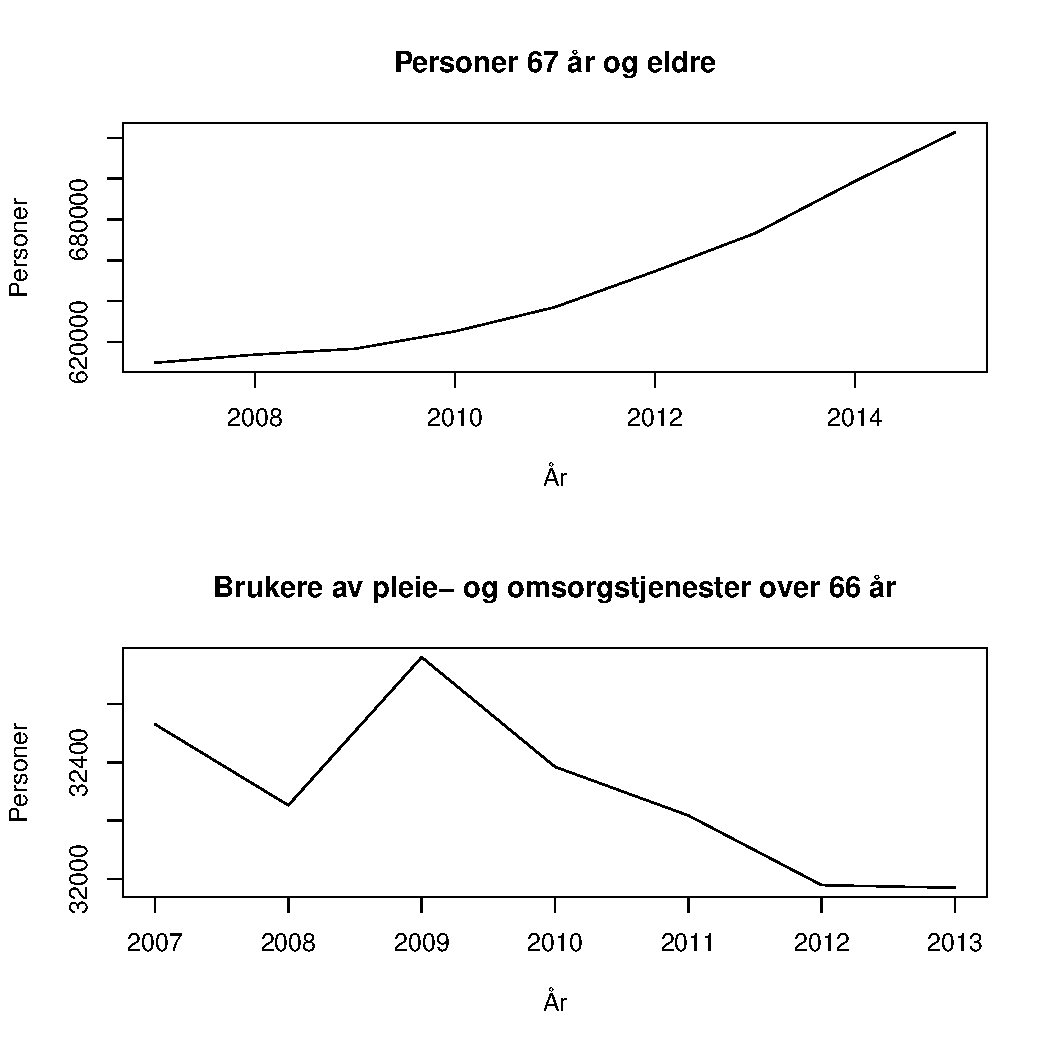
\includegraphics[width=\textwidth]{plots/eldre.pdf}
  \caption{Eldrebølgen visualisert, men ser ikke ut til å påvirke antall som
    trenger pleie- og omsorgstjenester. Tallgrunnlag fra Statistisk Sentralbyrå
  \cite{iplos.2013}}
  \label{fig.eldre}
\end{figure}
\clearpage

Alt dette viser at vi snakker om et ganske homogent marked (jmf.~<<market
differentiation>> \cite[s.~510]{bessant}).  Det er få forskjeller mellom
aktørene.  Dette kan dessverre tyde på lav avkastning og er et problem for
resultatene på budsjettene våre.  Men på den andre siden er det også et
nisjemarked og kan fremdeles være lukrativt. Vi har rett og slett ikke nok
kunnskap til å vite på forhånd om strategien vår vil fungere. 

Vi har imidlertid satset på innovasjon i et marked hvor det finnes lite.  Men
med innovasjon som våpen kan vi kanskje klare å komme oss inn på markedet, og
vi satser både på produkt med en tilhørende prosesseffektivisering. Vi kan
dermed lede en forandring i markedet og endre kundens forventninger til hva en
trygghetsalarm skal tilby.  Det er lav terskel for å lage en fullstendig
\textit{prototype}, og det kan være nok til å få dratt i gang forskning- og
uttestingsprogram med en kommune. Men det er en lang og dyr vei fra prototype
til salgsklart produkt.

Dersom vi klarer å holde foten i dørsprekken lenge nok til å etablere oss har
vi en fordel med en plattform som gjør at vi kan lansere produkter lynkjapt.
Når all kompleksiteten ligger på tjenersiden i programvare kan vi hypotetisk
sett utvikle en ny funksjon på en helg og lansere det til alle eksisterende
kunder på mandag. Dette er mulig fordi vi jobber med programvare, som har langt
kortere publiseringstid enn maskinvare. 

Konkurrentene våre må derimot designe ny maskinvare, bestille det fra Asia,
montere det, teste det, få elektronikkgodkjenninger og \textit{så} kan de
lansere. Dette gir oss en utrolig spennende mulighet til å utkonkurrere de
store. En velkjent strategi er <<planned obsolescence>> \cite{planned.obs}, som
i opprinnelig forstand går ut på å få kunden til å erstatte gamle produkt med
nye ved hele tiden å tilby nytt design, ny funksjonalitet og så videre.


% Ta med notater fra alt annet, spesielt om "viability", altså hvor realistisk
% det er, farer, osv. MÅ også ta med ting fra pensum!

% Husk "planned obsolesence", "minimum viable product", evt "exit-strategier"
% (mer osm i pivot-alternativ).

% Skim også gjennom boken

%\section{Risikomoment}

%\section{Prising}
